\documentclass[10pt]{article}

\usepackage[a4paper,margin=0.65in]{geometry}
\usepackage[utf8]{inputenc}
\usepackage{graphicx}
\usepackage{titlesec}
\usepackage{fancyhdr}
\usepackage{color}
\usepackage{parskip}
\usepackage{helvet}
\usepackage{longtable}
\usepackage{hyperref}
\usepackage{float}
\usepackage{caption}
\usepackage{lastpage}
\usepackage{array}
\usepackage{ragged2e}
\usepackage{makecell}
\usepackage{tabularx}
\usepackage[table]{xcolor}
\usepackage{colortbl}
\usepackage{placeins} % para FloatBarrier

% Colores para tablas
\definecolor{headergray}{gray}{0.9}
\definecolor{rowalt}{RGB}{245,245,255}

% Fuente sans-serif
\renewcommand{\familydefault}{\sfdefault}

% Encabezado
\pagestyle{fancy}
\fancyhf{}
\lhead{
\includegraphics[height=0.7cm]{images/logo_unit.png}}
\rhead{\textbf{UNIT Relay Module v1.0}}
\lfoot{Product Brief}
\rfoot{\thepage\ | \pageref{LastPage}}

% Estilo de secciones
\titleformat{\section}{\bfseries\large\sffamily}{}{0em}{}
\titleformat{\subsection}{\bfseries\normalsize\sffamily}{}{0em}{}
\titlespacing*{\section}{0pt}{1.2em}{0.5em}
\titlespacing*{\subsection}{0pt}{0.8em}{0.4em}

\title{}
\author{}
\date{}

\sloppy
\setlength{\emergencystretch}{3em}

\begin{document}

% Encabezado del documento
\noindent
\makebox[\textwidth][l]{%
    \begin{minipage}[t]{\textwidth}
        \Large \textbf{UNIT Relay Module Product Brief}\\[1.0em]
        \normalsize This dual-channel relay module safely interfaces microcontrollers with higher-voltage or high-current loads by separating control from power.\\[0.3em]
        \footnotesize\textsf{Version: 1.0 \hfill Modified: 2025-07-22 10:47}
    \end{minipage}%
}
\vspace{1em}
\hrule
\vspace{1.5em}

% Introducción con imagen
\section*{Introduction}
\vspace{0.5em}
\noindent
\begin{minipage}[t]{0.62\textwidth}
\setlength{\parskip}{0.75em}
\justifying
This dual-channel relay module isolates high-power operations from sensitive MCU logic. It supplies a dedicated 5V rail (JDVCC) for relay coils while using the VCC pin to match the MCU’s operating voltage (3.3V or 5V). A digital high on the IN pin triggers an optocoupler that switches the NO, NC, and COM contacts. LED indicators provide immediate feedback on power and control status.
\end{minipage}
\hfill
\begin{minipage}[t]{0.35\textwidth}
\centering
\vspace{-0.5em}
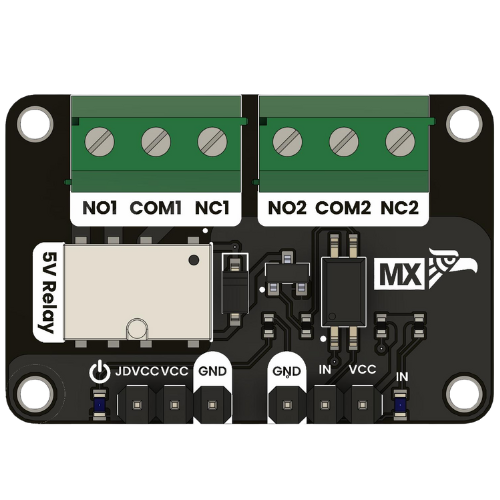
\includegraphics[height=4.2cm,keepaspectratio]{../../hardware/resources/img/relay_module.png}
\end{minipage}

\vspace{1.0em}
\FloatBarrier % evita que la imagen flote sobre el siguiente bloque



% Secciones técnicas
\section*{Functional Description}
- The module includes two independent electromechanical relays, each controlled through optocouplers for complete electrical isolation between control logic and relay coil voltage.\\ 
- A dedicated power rail (JDVCC) provides 5V specifically to energize the relay coils, while a separate VCC pin supplies 3.3V or 5V to the optocoupler input stage.\\ 
- Each relay channel is triggered via an active-high digital input signal (IN1, IN2) from the microcontroller.\\ 
- The relay outputs provide access to a set of contacts: Normally Open (NO), Normally Closed (NC), and Common (COM).\\ 
- When triggered, the relay switches the contacts, allowing control of external AC/DC loads while protecting the MCU from high-voltage transients.\\ 
- LED indicators (LED PWR and LED IN) provide immediate visual feedback of power and activation status.\\ 

\section*{Electrical Characteristics}
- Operating voltage (logic side): 3.0 V – 5.5 V (via VCC pin)\\ 
- Relay coil voltage: 5 V nominal (via JDVCC)\\ 
- Trigger current per channel: 2–15 mA depending on input logic level\\ 
- Contact rating: Up to 0.3 A - 125 VAC or 1 A - 30 VDC\\ 
- Optocoupler logic threshold: Compatible with 3.3 V and 5 V logic\\ 

\section*{Features}
- Dual-channel electromechanical relay outputs\\ 
- Optical isolation between control and power stages\\ 
- Dedicated 5V relay coil supply (JDVCC)\\ 
- 3.3V or 5V logic compatibility (VCC)\\ 
- LED indicators for control signal and power presence\\ 
- Breakout access to NO, NC, and COM terminals per channel\\ 



\section*{Applications}
- Home automation and IoT-based appliance control\\ 
- Industrial machinery switching\\ 
- Smart lighting systems\\ 
- Motor or actuator control\\ 
- Security and alarm systems\\ 

\vspace{1em}



\section*{Settings}

\subsection*{Interface Overview}
\rowcolors{2}{white}{rowalt}
\begin{tabularx}{\textwidth}{|c|c|>{\RaggedRight\arraybackslash}X|}
\hline
\rowcolor{headergray}
Interface & Signals / Pins & Typical Use \\
\hline
Power & JDVCC, VCC, GND & Power relay coils and optocoupler driver circuit \\
Control & IN1, IN2 & Trigger signals from MCU \\
Output & NO1, COM1, NC1 / NO2, COM2, NC2 & Switching terminals for AC/DC load \\
Indicators & LED (PWR), LED (IN) & Visual status of power and input activation \\
\hline
\end{tabularx}


\subsection*{Supported Pins}
\rowcolors{2}{white}{rowalt}
\begin{tabularx}{\textwidth}{|c|c|>{\RaggedRight\arraybackslash}X|}
\hline
\rowcolor{headergray}
Symbol & I/O & Description \\
\hline
JDVCC & Input & 5V supply input for relay coil energization \\
VCC & Input & Logic voltage input (3.3V or 5V) \\
GND & Input & Shared ground for logic and relay power \\
IN1 & Input & Control signal to activate relay 1 \\
IN2 & Input & Control signal to activate relay 2 \\
NOx & Output & Normally open contact (connected when active) \\
NCx & Output & Normally closed contact (disconnected when active) \\
COMx & Output & Common terminal for relay switching \\
\hline
\end{tabularx}




% Tabla principal
\section*{Pin \& Connector Layout}
\rowcolors{2}{white}{rowalt}
\begin{tabularx}{\textwidth}{|c|>{\RaggedRight\arraybackslash}X|}
\hline
\rowcolor{headergray}
Signal & Description \\
\hline
JDVCC & +5V supply to energize relay coils \\
VCC & MCU logic voltage (3.3V or 5V) for the optocoupler/driver circuit \\
IN & MCU input to activate relay channel 1 \\
NO1 & Relay 1 normally open contact \\
COM1 & Relay 1 common terminal \\
NC1 & Relay 1 normally closed contact \\
NO2 & Relay 2 normally open contact \\
COM2 & Relay 2 common terminal \\
NC2 & Relay 2 normally closed contact \\
LED PWR & Indicator LED for power (active when JDVCC is present) \\
LED IN & Indicator LED showing active input from the MCU \\
\hline
\end{tabularx}


% Imágenes adicionales
\FloatBarrier
\newpage
\vspace*{3em}
\section*{Block Diagram}
\vspace{1em}
\begin{center}
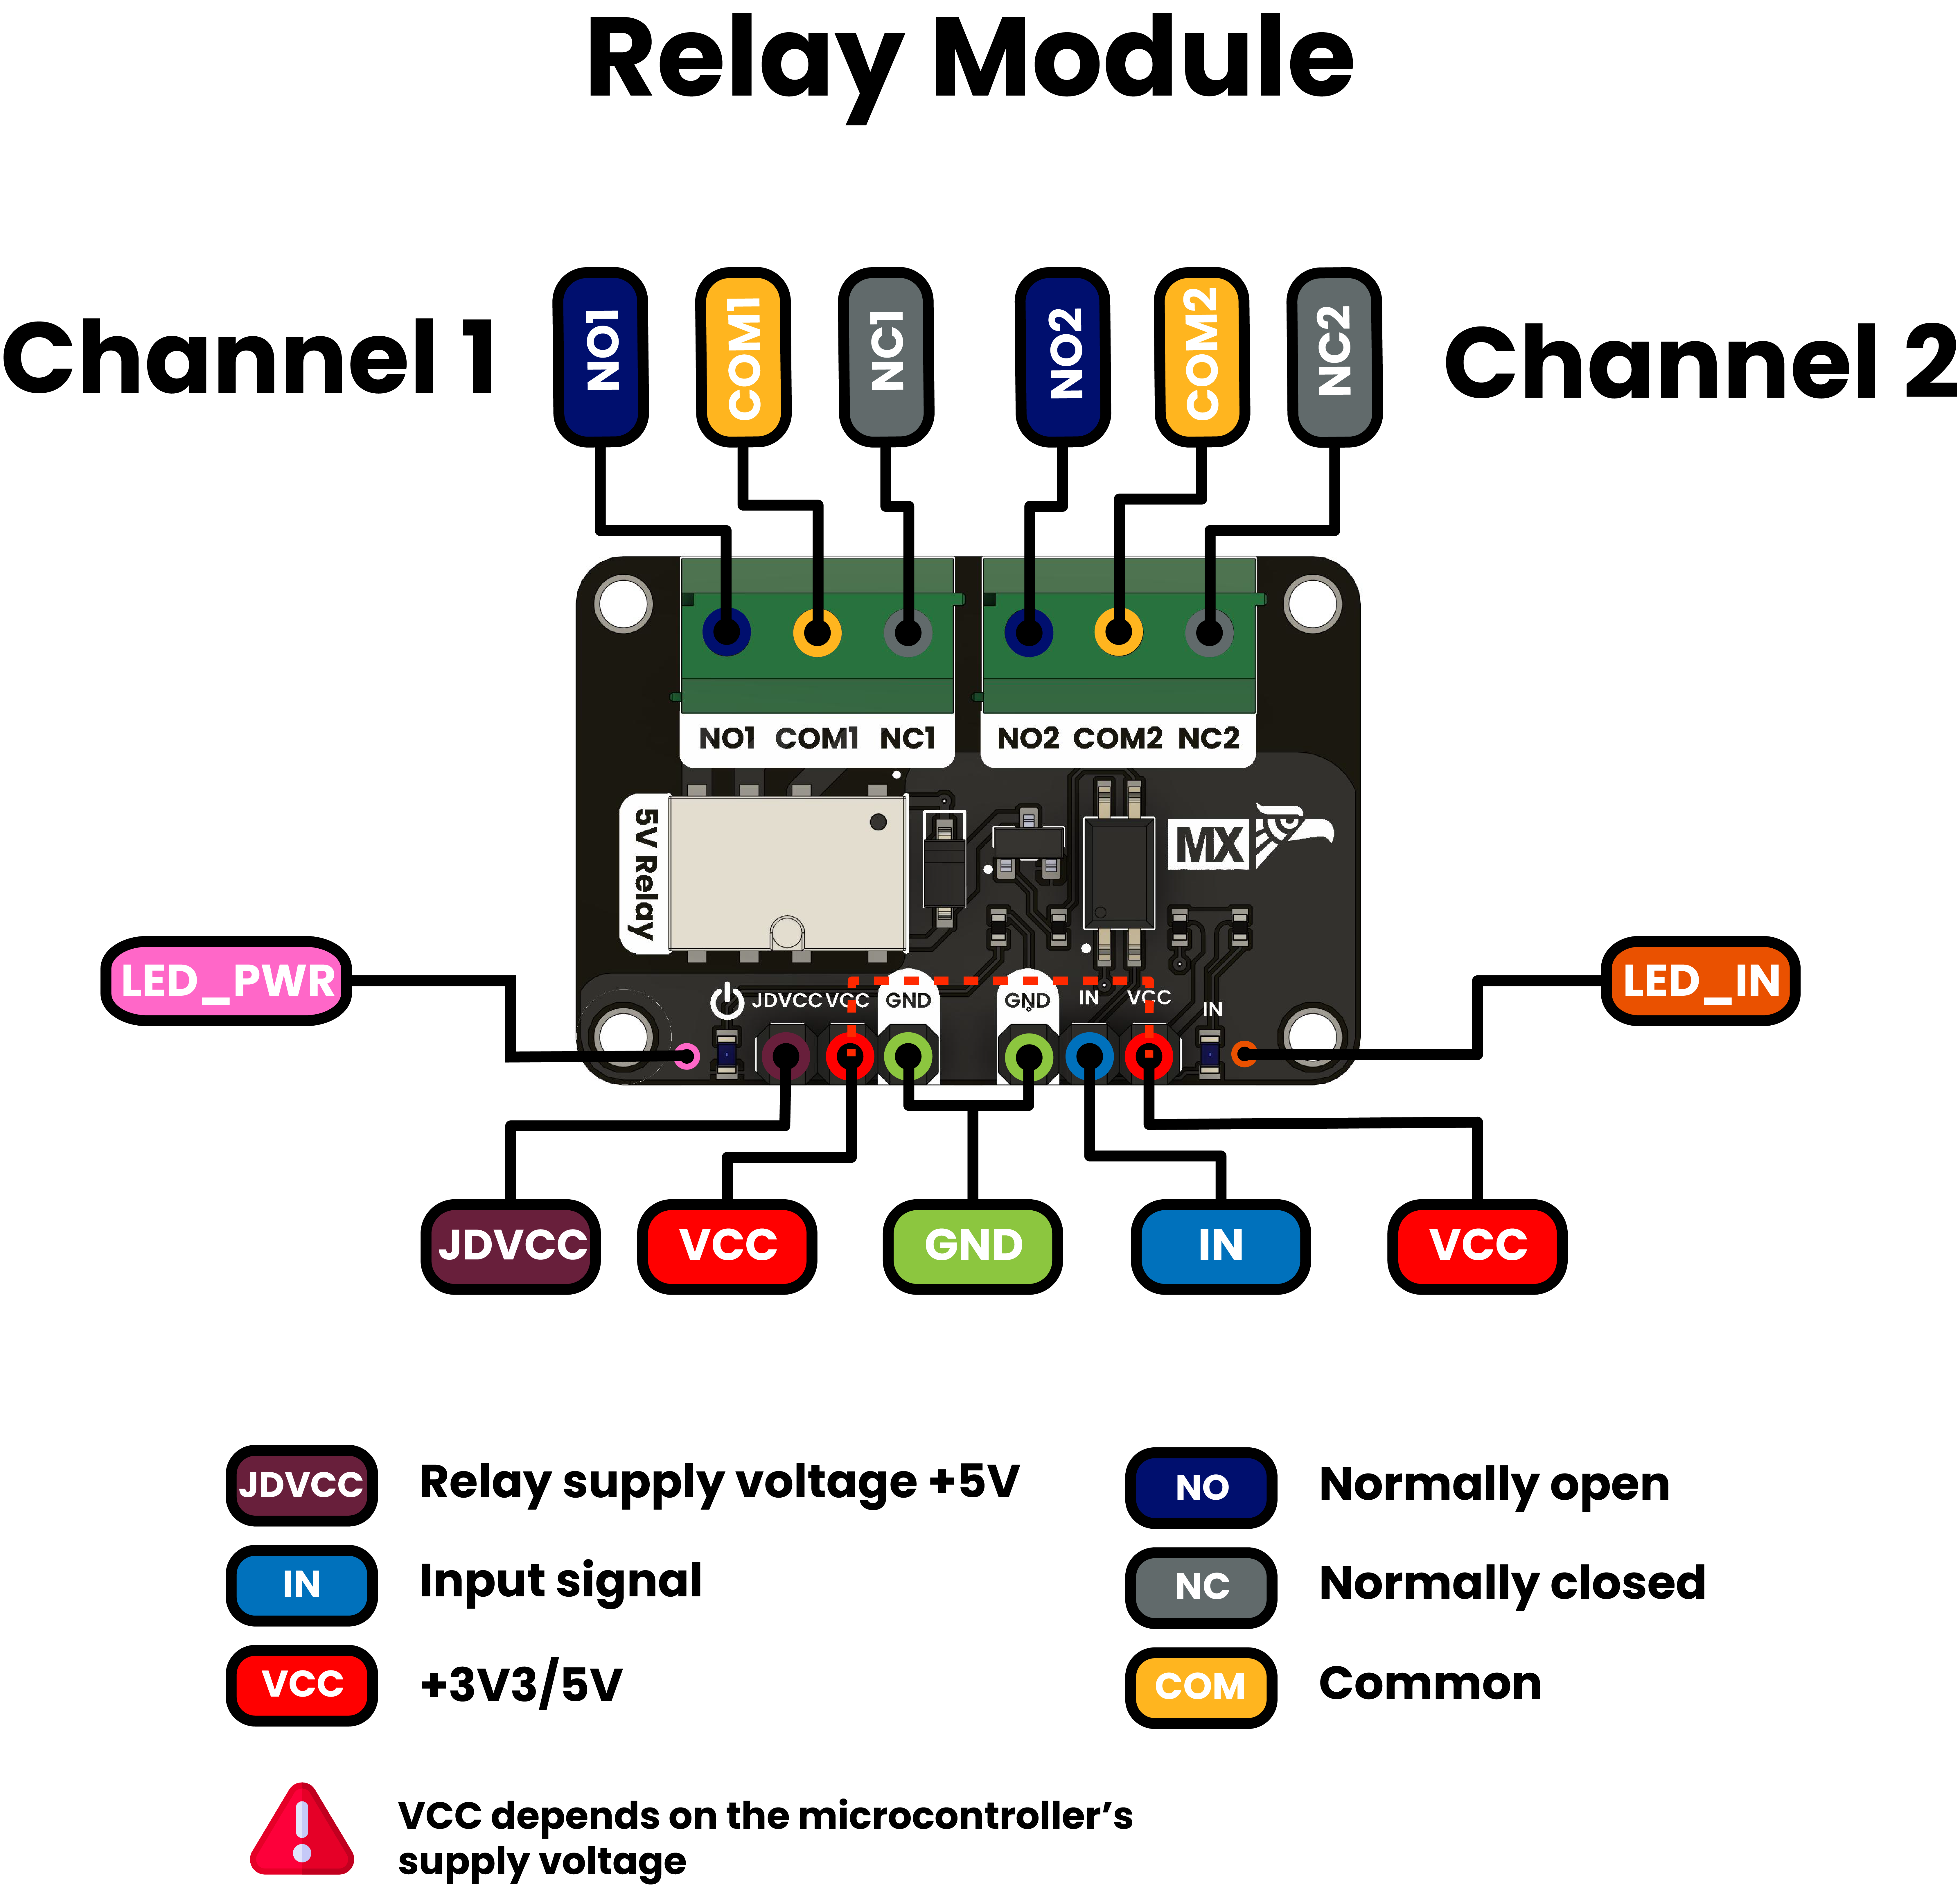
\includegraphics[width=0.75\textwidth,keepaspectratio]{../../hardware/resources/unit_pinout_v_0_0_1_ue0082_relay_en.png}
\end{center}
\newpage
\vspace*{3em}
\section*{Dimensions}
\vspace{1em}
\begin{center}
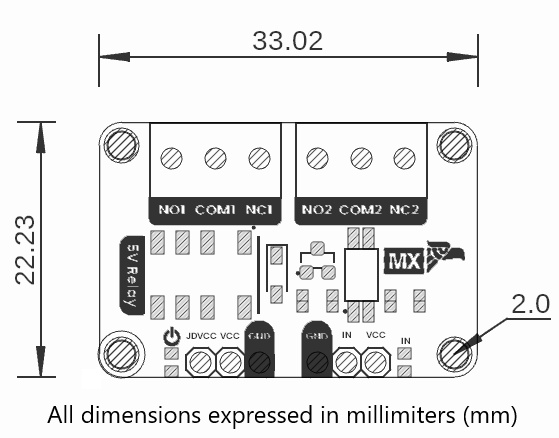
\includegraphics[width=0.75\textwidth,keepaspectratio]{../../hardware/resources/unit_dimension_v_0_0_1ue0082_modulo_rele_g6k_.png}
\end{center}



% Uso
\section*{Usage}
\begin{itemize}
\item Arduino AVR
\item Raspberry Pi RP2040
\item STM32
\item NRF
\item PY32
\item MAX II
\end{itemize}

% Descargas
\section*{Downloads}

\begin{itemize}
\item \href{unit_sch_v_0_0_1ue0082_modulo_rele_g6k_.pdf}{Schematic PDF}
\end{itemize}


% Compra
\section*{Purchase}
\begin{itemize}
\item \href{https://www.uelectronics.com}{Buy from UNIT Electronics}
\end{itemize}

\end{document}
